\chapter{Visão Geral}


Veículos aéreos não tripulados (VANTs) são aeronaves equipadas com sistemas embarcados, sensores e atuadores que permitem a realização de voos autônomos ou remotamente controlados. Eles são comumente classificados em dois grupos: veículos de asas rotativas, como helicópteros e quadrotores, e veículos de asas fixas, como aviões. 

Há diversas aplicações para VANTs, alguns exemplos são:

\begin{itemize}
	\itemsep0em
	\item Pulverização de culturas;
	\item Condução de rebanhos;
	\item Monitoramento de estradas;
	\item Inspeção da linhas de energia;
	\item Entrega de suprimentos em locais de difícil acesso.
\end{itemize}

Este trabalho está associado ao ProVANT\footnote{provant.paginas.ufsc.br}. O ProVANT consiste em uma parceria entre a Universidade Federal de Santa Catarina e a Universidade Federal de Minas Gerais, com o objetivo de realizar pesquisas e desenvolver novas tecnologias para aperfeiçoar o desempenho de VANTs. Neste contexto, atualmente, o ProVANT está focado no desenvolvimento de VANTs Tilt-rotor.  O Tilt-rotor está ilustrada na Figura \ref{vant.jpg} e é uma aeronave que possui configuração híbrida, portanto apresenta as principais vantagens das aeronaves de asa fixa e de asa rotativa, como por exemplo consumo reduzido de energia em voos de cruzeiro e decolagem e pouso na vertical. Ele pode operar tanto em ambientes fechados quanto abertos.

\begin{figure*}[!ht]
	\centering
	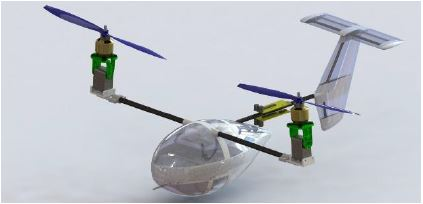
\includegraphics[width=0.8\textwidth]{figuras/VANT3.jpg}
	\caption{Tilt-rotor}
	\label{vant.jpg}
\end{figure*}

Com o intuito de fornecer uma ferramenta de testes para algoritmos e estratégias de controle voltados para vants, desenvolveu-se o simulador ProVANT. Pretende-se, dessa forma, reduzir de custos de projeto e tempo necessário para validação de novas tecnologias.

\section{Simuladores}

Simuladores voltados para aplicações de vants podem ser encontrados de duas maneiras: simuladores de voo e simuladores robóticos.

Simuladores de voo são ambientes desenvolvidos na maioria das vezes para treinamento de pilotos e/ou para desenvolvimento de jogos de aviões e helicópteros. X-plane e FlightGear são os simuladores mais utilizados por cientistas e profissionais da indústria aeronáutica.

Os simuladores robóticos são ambientes de desenvolvimento de simulação de robôs. O simulador Gazebo e o simulador V-rep são dois exemplos que se destacam nesta classe. Os simuladores robóticos são utilizados para testes e validação de algoritmos de controle e planejamento de trajetória. Estes trabalham com modelos de dinâmica multi-corpo com base nos conceitos de elos e juntas. 

A seguir será feito uma revisão bibliográfica sobre aplicações de vants em: i) X-plane; ii) Flightgear; iii) Gazebo; iv) V-rep.


\subsection{X-plane}

O X-plane\footnote{www.x-plane.com} é um simulador de voo multiplataforma (Linux, MAC e Windows) com a credencial da FAA (Administração Federal de Aviação) que simula voos baseado nos efeitos das forças sobre as múltiplas seções de uma aeronave. O X-plane inclui mais de 30 exemplares de aeronaves disponíveis para simulação e possui a capacidade de customização de cenário e importação de novas aeronaves. Esse simulador permite ao usuário configurar diferentes superfícies de controle aerodinâmico e realizar comunicação externa via protocolo UDP. Além disso, realiza tratamento de diferentes condições atmosféricas de acordo com a altitude. No entanto, o simulador apresenta como desvantagens ser um software proprietário, incapaz de simular múltiplos objetos de simulação no mesmo computador e de realizar simulações com modelos multi-corpos.

Em \cite{Figueiredo2012} foi modelado e simulado um quadrotor no simulador X-plane. A modelagem baseou-se numa aeronave desenvolvida por um grupo de pesquisa do Instituto Tecnológico da Aeronáutica, sendo utilizado o Matlab/Simulink para realizar o controle automático do quadrotor. Em \cite{Castro2014} e \cite{Garcia2010}, desenvolveu-se um ambiente de simulação para múltiplos VANTs na configuração quadrotor de forma semelhante a \cite{Figueiredo2012}. No entanto, devido ao elevado esforço computacional exigido pelo simulador, fez-se necessário a utilização de diversos computadores para a aplicação. Já em \cite{Bittar2014}, realizou-se uma simulação \textit{Hardware-in-the-loop} no X-plane de um veículo de asas fixas. Neste trabalho, o comportamento mecânico e aerodinâmico do VANT na configuração avião foi simulado pelo X-plane e o respectivo controlador foi implementado por um sistema embarcado. A comunicação entre o simulador X-plane e o controlador foi realizada através de comunicação serial, sendo que o último recebe do simulador em tempo real os dados dos sensores e, após processamento do controlador, reenvia os sinais de controle.

\subsection{FlightGear}

O FlightGear\footnote{www.flightgear.org} é um software de simulação de voo multiplataforma de código aberto. É extensível e utiliza três modelos de dinâmica de voo: JSBSim,YASim e UIUC. 

JSBSim é um modelo de dinâmica de voo genérico com seis graus de liberdade, onde a aeronave é modelada utilizando um arquivo XML, em que se define as propriedades de massa, aerodinâmica e controle de voo. YASim é um modelo de dinâmica de voo que simula o efeito da corrente de ar nas diferentes partes da aeronave. Por fim, o UIUC é um modelo de dinâmica de voo que engloba em simulação um modelo de aerodinâmica não-linear. Ele resulta em simulações com maior grau de realismo, sobretudo em situações de atitudes extremas, como estol e elevado ângulo ataque.

O simulador possui um banco de modelos e cenários disponíveis (cerca de 20.000 aeroportos reais), é capaz de simular de forma precisa falhas de sistemas e instrumentos aeronáuticos. Porém, é incapaz de emular modelos multi-corpos e de realizar simulações com mais de um modelo concomitantemente.    

O FlightGear foi utilizado por \cite{Sorton2005} como simulador para VANTs na configuração avião, e como controlador foi utilizado Matlab/Simulink. Já em \cite{Butt01052016}, foi desenvolvido um algoritmo \textit{offline} de geração de trajetórias 4D (tempo, longitude, latitude e altitude) para um VANT de asas fixas, sendo utilizado o simulador FlightGear para validá-lo.

\subsection{Gazebo}

Gazebo\footnote{www.gazebosim.org} \'e um software livre de simula\c c\~ao rob\'otico desenvolvido pela OSRF (Open Source Robotics Foundation), capaz de simular eficientemente popula\c c\~oes de objetos em cen\'arios complexos, sejam eles ambientes externos ou internos.

Esse simulador é apropriado para simulações com múltiplos objetos e detecção de colisão, sendo estes constituídos de um ou mais corpos. Esse sistema possui um banco de sensores considerável (ao todo são 12, contendo a capacidade de criar sensores customizados) e permite ao usuário incluir novos cenários e objetos de simulação através de arquivos XML. Além disso, possibilita que o usuário realize simulações na nuvem, por exemplo em servidores da Amazon. 

Algumas simulações de VANTs utilizando o Gazebo são encontradas na literatura. Em \cite{Nagaty2013}, projetou-se um controlador em cascata utilizando a estratégia de controle não linear  \textit{Backstepping} para a malha de controle interna e um controlador PD na malha externa. Ademais, validou-se o controlador projetado utilizando ROS (Robotic Operating System) e Gazebo. Já em \cite{Martinez2013}, desenvolveu-se um sistema de visão 3D para helicópteros, o qual foi utilizado numa simulação com o Gazebo.

\subsection{V-REP}

V-rep\footnote{www.coppeliarobotics.com} \'e um software de simula\c c\~ao rob\'otico multi-plataforma, desenvolvido pela Coppelia Robotics, capaz de simular popula\c c\~oes de objetos multi-corpos. É um sistema com interface amigável e suporte a várias linguagens de programação, sendo capaz de tratar colisões entre objetos de simulação, criar novos cenários e importar novos modelos. 

Apesar de sua vasta utilização para sistemas robóticos, pouco se encontra sobre o uso do V-REP com VANTs. Em \cite{7158723}, apresentou-se um ambiente de simulação desenvolvido com V-REP e ROS. Esse cenário foi utilizado para sintonia de uma abordagem de controle para um VANT VTOL (acrônimo para  \textit{Vertical Take-Off and Landing}, que significa decolagem e aterrissagem vertical) baseada em visão computacional. Foi proposto um algoritmo de controle baseado em redes neurais, adotando um estimador de pose com base no conhecimento da posição do local de decolagem. 


\section{Requisitos de projeto software}

%\subsection{Requisitos de Projeto}
%\markright{\thesection ~~~ Objetivos}
%label{objetivos}

No inicio do projeto de desenvolvimento do simulador ProVANT, definiu-se os seguintes requisitos não funcionais:

\begin{itemize}
	\itemsep0em
	\item[i)] Funcionar sobre sistema operacional Ubuntu/Linux;
	\item[ii)] Ter licen\c ca de software livre;
	\item[iii)] Ser capaz de realizar tratamento de colis\~oes;
	\item[iv)] Emular modelos multi-corpos;
	\item[v)] Incluir modelos de simulação com projeto CAD (projetos realizados com auxílio de computadores).
\end{itemize}	


Quanto aos requisitos funcionais, definiu-se:

\begin{itemize}
	\itemsep0em
	\item[i)] Interface gráfica para configuração de elementos de simulação;
	\item[ii)] Conjunto de instrumentos para medição e controle de variáveis físicas; 
	\item[iii)] Controlador a ser configurado pelo usuário. 
\end{itemize} 

Tendo em vista os requisitos não funcionais do projeto, os simuladores de voo descritos não são adequados, pois estes não são capazes de trabalhar com modelos de simulação multi-corpos. Já os simuladores robóticos descritos atendem a quase todos esses requisitos. Ambos funcionam no sistema operacional Ubuntu/Linux, são capazes de emular modelos multi-corpos e fazem tratamento de colisões. 


Entre os simuladores robóticos, o Gazebo é único exemplar que apresenta licença de software livre e acesso externo aos parâmetros do modelo via arquivo XML, facilitando a criação, modificação e armazenamento de modelos de simulação. Porém a característica determinante para a escolha do simulador a ser utilizado foi a existência de suporte pelo Gazebo, no início deste trabalho (Setembro/2015), à atuação de juntas rotativas via conjugado mecânico, o que não ocorria no V-REP. Portanto, devido a essas características, o Gazebo foi o simulador selecionado como base de software de simulação.

\section{Softwares utilizados}

Além do software de simulação Gazebo, utilizou-se outros 2 componentes de software para o desenvolvimento do simulador ProVANT: a plataforma de desenvolvimento QT e o ROS (Robot Operating System). A seguir será dado uma visão geral de cada componente.

\subsubsection{QT}

Parte do ambiente de simulação ProVANT foi desenvolvido na linguagem C++, utilizando a IDE QtCreator e bibliotecas da plataforma QT versão 5. Qt é uma plataforma de desenvolvimento de aplicações multi-plataforma (hardware e software) com ou sem interface gráfica. O Qt é desenvolvido atualmente pela \textit{The Qt Company} e disponibiliza diversos recursos aos programadores, tais como acesso a banco de dados SQL, análise XML, análise JSON, gerenciamento de threads e suporte de rede.

\subsubsection{ROS}

Robot Operating System (ROS) é uma plataforma de desenvolvimento de código aberto baseado em Linux para desenvolvimento robótico. O ROS provê funcionalidades que vão desde abstração de hardware e controle em baixo nível de dispositivos até navegação, planejamento de movimento e simulação de alto nível. O sistema foi desenvolvido inicialmente em 2007 no Laboratório de Inteligência Artificial de Stanford e agora é mantido por Willow Garage, um centro de pesquisa em robótica e incubadora.

As aplicações ROS são organizadas em estruturas chamadas Stacks, que agregam os Pacotes (em inglês, Packages) onde se encontram os executáveis, códigos-fonte e bibliotecas. Cada um desses níveis contém um arquivo de manifesto (chamdo ''package.xml'') responsável pela descrição do conteúdo, facilitando o compartilhamento com a comunidade científica. 

O ROS é um sistema descentralizado que permite que aplicações sejam executadas de forma distribuída entre as máquinas. Quando um arquivo executável de um pacote é iniciado, este origina um ou mais nós. Os nós representam processos individuais que se comunicam através dos chamados tópicos. Essa estrutura abstrai um sistema de troca de mensagens assíncrono baseado em sockets. Os nós podem atuar como publicadores em múltiplos tópicos simultaneamente. Enquanto publicadores, um único tipo de dado pode ser postado em um certo tópico, normalmente à uma taxa constante.

O elemento final na estrutura do ROS é o chamado ROS Core (roscore), que é executado em uma única máquina e atua como o DNS (Domain Name System). Cada nó deve receber um identificador ROS Core (Uniform Resource Identifier - URI) para que, durante a execução, os nós possam notificar ao ROS Core que eles existem. Essa estratégia permite que os nós se comuniquem através de conexões remotas e locais online.

\section{Organização do manual}

O Texto está organizado como a seguir:

\begin{enumerate}
	\item Este capítulo introduz dá uma visão geral sobre o simulador ProVANT
	\item O segundo capítulo apresenta a estrutura do ambiente de simulação ProVANT;
	\item O terceiro capítulo organização do projeto de software, descrevendo a localização de arquivos e diretórios;
	\item O quarto capítulo descreve detalhes do projeto relativo ao simulador Gazebo. Será abordado sobre modelos, cenários e plugins;
	\item O quinto capítulo descreve detalhes do Controlador;
	\item O sexto capítulo descreve detalhes da Interface gráfica;
	\item O sétimo capítulo descreve como é o processo de inicialização de uma instância de simulação.
	\item O apêndice A descreve como se configurar um arquivo ''CMakeLists.txt'' genérico.
	\item O apêndice B descreve como se configurar um arquivo ''package.xml'' genérico.
\end{enumerate}




